\documentclass[12pt, a4paper, oneside]{article}
\usepackage{amsmath, amsthm, amssymb, appendix, bm, graphicx, float, subfigure, caption, hyperref, mathrsfs, indentfirst}

\usepackage{CJKutf8}

\title{\textbf{Math Notes}}
\author{Haotian Deng}
\date{}

\linespread{1.5}
\setlength{\parindent}{2em}

%\usepackage{setspace}
%\setstretch{1.8} 

\begin{document}

\maketitle

\begin{CJK*}{UTF8}{gbsn}


%%%%%%%%%%%%%%%%%%%%%%%%%%
\newpage
\section{静态(均衡)分析}
%
\subsection{对角矩阵}
%%
\textbf{对角矩阵}:非对角线元素均为0的对称矩阵。
$$
x=\left[\begin{array}{l}x_{1} \\ x_{2}\end{array}\right]
\quad
A=\left[\begin{array}{cc}a_{11} & 0 \\ 0 & a_{22}\end{array}\right]
$$
\begin{itemize}
	\item 平方和:
		$
		x^{\prime}x=
		\left[\begin{array}{ll}x_{1} & x_{2}\end{array}\right]
		\left[\begin{array}{l}x_{1} \\ x_{2}\end{array}\right]
		=x_{1}^{2}+x_{2}^{2}
		$
	\item 加权平方和:
		$
		x^{\prime}Ax=
		\left[\begin{array}{ll}x_{1} & x_{2}\end{array}\right]
		\left[\begin{array}{cc}a_{11} & 0 \\ 0 & a_{22}\end{array}\right]
		\left[\begin{array}{l}x_{1} \\ x_{2}\end{array}\right]
		=a_{11} x_{1}^{2}+a_{22} x_{2}^{2}
		$
\end{itemize}

%
\subsection{拉普拉斯展开}
%%
\noindent
\textbf{拉普拉斯展开(按行/列展开)}:
$
|B|=\sum_{j=1}^{n}b_{i, j}\left|C_{ij}\right|=\sum_{i=1}^{n}b_{i, j}\left|C_{i,j}\right|
$
%%
\begin{itemize}
	\item \textbf{子式}:删除行列式$|A|$的第$i$行第$j$列而得到的子行列式$|M_{ij}|$。
	\item \textbf{余子式}:$\left|C_{ij}\right|=(-1)^{i+j}\left|M_{ij}\right|$。
\end{itemize}

%
\subsection{矩阵的秩}
%%
\begin{itemize}
	\item 矩阵的\textbf{秩}:\textbf{线性无关}的\textbf{最大}行/列数。
	\item $r(A) \leqslant \min \{m, n\}$。
	\item \textbf{非奇异矩阵}$M_{n\times n}$的\textbf{秩}必为$n$:$r(A)=n$。
	\item $r(A B) \leqslant \min \{r(A), r(B)\}$。
	\item $B$为\textbf{非奇异矩阵},则$r(A)=r(AB)$或$r(A)=r(BA)$。
\end{itemize}

%
\subsection{克莱姆法则}
%%
\noindent
按\textbf{异行余子式}进行\textbf{拉普拉斯展开}的行列式为\textbf{0}:
$$
\sum_{j=1}^{n}a_{i, j}\left|C_{i^{\prime}, j}\right|=\sum_{i=1}^{n}a_{i, j}\left|C_{i, j^{\prime}}\right|=0
$$
%%
\noindent
\textbf{伴随矩阵}$\text{adj} A$:
给定\textbf{非奇异矩阵}
$A_{n\times n}=\left[\ |a_{ij}|\ \right]$,
$|A|\neq 0$,以\textbf{余子式}$\left|C_{i, j}\right|$
置换$A$中每一个元素$a_{ij}$而形成一个
\textbf{余子式矩阵}$C_{n\times n}=\left[\ |C_{ij}|\ \right]$,
则\textbf{转置矩阵}$C^{\prime}$为$A$的
\textbf{伴随矩阵},即$C^{\prime}_{n\times n}=\text{adj}A=\left[\ |C_{ji}|\ \right]$。

$$\text{\textbf{矩阵的逆}:}A^{-1}=\frac{\text{adj}A}{|A|}$$
%%
\noindent
方程组$A_{n\times n}x_{n\times 1}=d_{n\times 1}$($\textbf{A}$为\textbf{非奇异矩阵})的\textbf{解}:$x^{*}=A^{-1} d=\frac{\text{adj} A}{|A|}\cdot d$
$$
\textbf{克莱姆法则:}
x_{j}^{*}=\frac{\left|A_{j}\right|}{|A|}=
\frac{1}{|A|}
\left[\begin{array}{cccccc}
a_{11} & a_{12} & \cdots & d_{1} & \cdots & a_{1n} \\
a_{21} & a_{22} & \cdots & d_{2} & \cdots & a_{2n} \\
\vdots & \vdots &&  \vdots &&  \vdots \\
a_{n1} & a_{n2} & \cdots & d_{n} & \cdots & a_{nn}
\end{array}\right]
$$
%%%%%%%%%%%%%%%%%%%%%%%%%%
\newpage
\section{比较静态分析}

%
\subsection{隐函数定理}
%%
\noindent
\textbf{雅可比行列式}:
$$
|J| \equiv\left|\frac{\partial\left(y_{1}, y_{2}, \cdots, y_{n}\right)}{\partial\left(x_{1}, x_{2}, \cdots, x_{n}\right)}\right| \equiv\left|\begin{array}{cccc}\frac{\partial y_{1}}{\partial x_{1}} & \frac{\partial y_{1}}{\partial x_{2}} & \cdots & \frac{\partial y_{1}}{\partial x_{n}} \\ \cdots &\cdots &\cdots &\cdots  \\ \frac{\partial y_{n}}{\partial x_{1}} & \frac{\partial y_{n}}{\partial x_{2}} & \cdots & \frac{\partial y_{n}}{\partial x_{n}}\end{array}\right| \equiv\left|\begin{array}{ccc}f_{1} & \cdots & f_{n} \\ \vdots & & \vdots \\ f_{1}^{n} & \cdots & f_{n}^{n}\end{array}\right| 
$$

%%
\noindent\textbf{隐函数法则}:给定方程$F(y, x)=0$,
$$\frac{dy}{dx}=-\frac{F_x}{F_y}$$

%%
推广到联立方程组的情况:

$
\begin{array}{c}
F^{1}\left(y_{1}, \cdots, y_{n} ; x_{1}, \cdots, x_{m}\right)=0, \\ 
F^{2}\left(y_{1}, \cdots, y_{n} ; x_{1}, \cdots, x_{m}\right)=0, \\ 
\cdots \\ 
F^{n}\left(y_{1}, \cdots, y_{n} ; x_{1}, \cdots, x_{m}\right)=0.
\end{array}
$
$\Leftrightarrow$
$
\begin{aligned}
y_{1}&=f^{1}\left(x_{1}, \cdots, x_{m}\right), \\ 
y_{2}&=f^{2}\left(x_{1}, \cdots, x_{m}\right), \\  
 &\cdots    \\ 
y_{n}&=f^{n}\left(x_{1}, \cdots, x_{m}\right) .
\end{aligned}
$
\begin{itemize}
	\item 对所有$y$变量和$x$变量,\textbf{隐函数}$F^1,\cdots F^n$均具有\textbf{连续偏导数}。
	\item 在点$\left(y_{10}, \cdots, y_{n0} ; x_{10}, \cdots, x_{m0}\right)$满足上述联立方程组。
	\item \textbf{雅可比行列式}
	$
	|J| \equiv\left|\frac{\partial\left(F^{1}, \cdots, F^{n}\right)}{\partial\left(y_{1}, \cdots, y_{n}\right)}\right| \equiv\left|\begin{array}{cccc}\frac{\partial F^{1}}{\partial y_{1}} & \frac{\partial F^{1}}{\partial y_{2}} & \cdots & \frac{\partial F^{1}}{\partial y_{n}} \\ \frac{\partial F^{2}}{\partial y_{1}} & \frac{\partial F^{2}}{\partial y_{2}} & \cdots & \frac{\partial F^{2}}{\partial y_{n}} \\ \cdots &\cdots &\cdots &\cdots  \\ \frac{\partial F^{n}}{\partial y_{1}} & \frac{\partial F^{n}}{\partial y_{2}} & \cdots & \frac{\partial F^{n}}{\partial y_{n}}\end{array}\right| \neq 0
	$
\end{itemize}
$$
\left[
	\begin{array}{cccc}
		\frac{\partial F^{1}}{\partial y_{1}} & \frac{\partial F^{1}}{\partial y_{2}} & \cdots & \frac{\partial F^{1}}{\partial y_{n}} \\
		\frac{\partial F^{2}}{\partial y_{1}} & \frac{\partial F^{2}}{\partial y_{2}} & \cdots & \frac{\partial F^{2}}{\partial y_{n}} \\
		 \cdots &\cdots &\cdots &\cdots \\
		  \frac{\partial F^{n}}{\partial y_{1}} & \frac{\partial F^{n}}{\partial y_{2}} & \cdots & \frac{\partial F^{n}}{\partial y_{n}}
	\end{array}
\right]
\left[
	\begin{array}{c}
		\left(\frac{\partial y_{1}}{\partial x_{1}}\right) \\
		\left(\frac{\partial y_{2}}{\partial x_{1}}\right) \\
		\vdots \\
		\left(\frac{\partial y_{n}}{\partial x_{1}}\right)
	\end{array}
\right]
=
\left[
	\begin{array}{c}
		-\frac{\partial F^{1}}{\partial x_{1}} \\
		-\frac{\partial F^{2}}{\partial x_{1}} \\
		\vdots \\
		-\frac{\partial F^{n}}{\partial x_{1}}
	\end{array}
\right]
\Rightarrow
\left(\frac{\partial y_{j}}{\partial x_{1}}\right)=\frac{\left|J_{j}\right|}{|J|}, \quad(j=1,2, \cdots, n)
$$
%%%%%%%%%%%%%%%%%%%%%%%%%%
\newpage
\section{最优化}

%
\subsection{麦克劳林级数与泰勒级数}
%%
\noindent\textbf{$n$次多项式函数}:
$f(x)=a_{0}+a_{1} x+a_{2} x^{2}+a_{3} x^{3}+a_{4} x^{4}+\cdots+a_{n} x^{n}$
%%
$$
\textbf{麦克劳林级数:}
f(x)=\frac{f(0)}{0 !}
+\frac{f^{\prime}(0)}{1 !} x
+\frac{f^{\prime \prime}(0)}{2 !} x^{2}
+\frac{f^{\prime \prime}(0)}{3 !} x^{3}
+\cdots+\frac{f^{(n)}(0)}{n !} x^{n}
$$
%%
$$
\textbf{泰勒级数:}
f(x)=\frac{f(x_{0})}{0 !}
+\frac{f^{\prime}\left(x_{0}\right)}{1 !}\left(x-x_{0}\right)
+\frac{f^{\prime \prime}\left(x_{0}\right)}{2 !}\left(x-x_{0}\right)^{2}
+\cdots
+\frac{f^{(n)}\left(x_{0}\right)}{n !}\left(x-x_{0}\right)^{n} 
%%
$$
\textbf{任意函数展开:}
$$
\begin{aligned}
	\phi(x)=&
	\left[
	\frac{\phi\left(x_{0}\right)}{0 !}
	+\frac{\phi^{\prime}\left(x_{0}\right)}{1 !}\left(x-x_{0}\right)
	+\frac{\phi^{\prime\prime}\left(x_{0}\right)}{2 !}\left(x-x_{0}\right)^{2}
	+\cdots
	+\frac{\phi^{(n)}\left(x_{0}\right)}{n !}\left(x-x_{0}\right)^{n}
	\right]
	+R_{n} 
	\\ \equiv & P_{n}+R_{n}
\end{aligned}
$$
$$
R_{n}=\frac{\phi^{(n+1)}(p)}{(n+1) !}\left(x-x_{0}\right)^{n+1}
$$
$$
n=0
\quad\Rightarrow\quad
\phi(x)=P_{0}+R_{0}=\phi\left(x_{0}\right)+\phi^{\prime}(p)\left(x-x_{0}\right)
$$
$$
\Downarrow
$$
$$
\phi(x)-\phi\left(x_{0}\right)=\phi^{\prime}(p)\left(x-x_{0}\right)
$$
$$
\Downarrow
$$
$$
\begin{aligned}
f(x)  -f\left(x_{0}\right)&=f^{\prime}\left(x_{0}\right)\left(x-x_{0}\right)+\frac{f^{\prime \prime}\left(x_{0}\right)}{2 !}\left(x-x_{0}\right)^{2} \\
 & +\cdots+\frac{f^{(n)}\left(x_{0}\right)}{n !}\left(x-x_{0}\right)^{n}+\frac{f^{(n+1)}(p)}{(n+1) !}\left(x-x_{0}\right)^{n+1}
\end{aligned}
$$

%
\subsection{增长率}
%%
\noindent
变量$y=f(t)$的\textbf{瞬时增长率}为
$$
r_{y} \equiv \frac{\mathrm{d} y / \mathrm{d} t}{y}=\frac{f^{\prime}(t)}{f(t)}=\frac{\text{边际函数}}{\text{总函数}}
$$
变量$V=Ae^{rt}$的\textbf{瞬时增长率}为
$$
r_{V}=\frac{V^{\prime}(t)}{V(t)}=\frac{d\ln V}{dt}=\frac{d(\ln A+rt)}{dt}=r
\quad\quad(\frac{\ln V}{dt}=\frac{V^{\prime}(t)}{V(t)})
$$

%
\subsection{多变量函数极值}
%%
\noindent
\textbf{一阶条件}是极值存在的\textbf{必要条件},但不是\textbf{充分条件}。
\begin{itemize}
	\item \textbf{鞍点}:某一方向上的函数\textbf{极大值点},另一方向上是函数\textbf{极小值点}。
	\item \textbf{拐点}:函数\textbf{凹凸性}发生变化的点。
	\item \textbf{驻点(稳定点)}:函数\textbf{一阶导数为0}的点。
\end{itemize}

%%
\textbf{杨氏定理}:$f_{x y}=f_{y x}$ (两个交叉偏导数是连续的)
\newline

%%
\noindent
\textbf{二阶条件}
\begin{itemize}
	\item 极值的二阶\textbf{充分条件}:对于任意不同时为0的$\mathrm{d}x$和$\mathrm{d}y$,$\mathrm{d}^2z \gtrless 0$。
	\item 极值的二阶\textbf{必要条件}:对于任意不同时为0的$\mathrm{d}x$和$\mathrm{d}y$,$\mathrm{d}^2z \leq\geq 0$。
\end{itemize}

%
\subsection{二次型}
%%
$$
\begin{aligned}
	\mathrm{d}^{2} z 
	& = f_{x x} \mathrm{~d} x^{2}+2 f_{x y} \mathrm{~d} x \mathrm{~d} y+f_{y y} \mathrm{~d} y^{2}
	\\
	& \Downarrow
	\\
	q &
	= a u^{2}+2 h u v+b v^{2} 
	= 
	 \left[
		 \begin{array}{cc}u & v\end{array}
	 \right]
	 \left[
		 \begin{array}{cc}a & h \\ h & b\end{array}
	 \right]
	 \left[
		 \begin{array}{c}u \\ v\end{array}
	 \right]
\end{aligned}
$$
$$
\text{若}\ q \ \text{恒为}
\left\{
	\begin{array}{ll}
		\text{正} & (>0) \\
		\text{非负} & (\geqslant 0) \\
		\text{非正} & (\leqslant 0) \\
		\text{负} & (<0)
	\end{array}
\right.,
\quad
\text{则}\ q \ \text{为} 
\left\{
	\begin{array}{l}
		\text{正定} \\
		\text{半正定} \\
		\text{半负定} \\ 
		\text{负定}
	\end{array}
\right.
$$

%%
\noindent
\textbf{海塞行列式}:对称行列式(杨氏定理$f_{x y}=f_{y x}$)
$$
|H|
=\left|\begin{array}{cc}a & h \\ h & b\end{array}\right|
=\left|\begin{array}{ll}f_{x x} & f_{x y} \\ f_{y x} & f_{y y}\end{array}\right|
$$
二次型的判别:
$$
\left\{\begin{array}{l}f_{x x} \gtrless 0 \\ |H|>0\end{array}\right.
\quad\Longleftrightarrow\quad
\mathrm{d}^{2} z \text{为}\left\{\begin{array}{l}\text{正定} \\ \text{负定}\end{array}\right.
$$

%%
\noindent
\textbf{$n$-变量}二次型
$$
\begin{aligned}
	q\left(u_{1}, u_{2}, \cdots, u_{n}\right) 
	& =
	\sum_{i=1}^{n} \sum_{j=1}^{n} d_{i j} u_{i} u_{j} 
	\quad [\text{其中}d_{i j}=d_{ji}]
	\\ & =
	\underset{(1 \times n)}{u^{\prime}} \underset{(n \times n)}{D} \underset{(n \times 1)}{u} 
\end{aligned}
$$

\begin{itemize}
	\item \textbf{正定}的充要条件为:\textbf{主子式}均为正。
		$$
		\begin{array}{c}
			\left|D_{1}\right| \equiv d_{11}>0,
			\quad
			\left|D_{2}\right| \equiv 
				\left|
				\begin{array}{ll}d_{11} & d_{12} \\ d_{21} & d_{22}\end{array}
				\right| >0, 
			\quad \cdots, 
			\quad
			\left|D_{n}\right| \equiv\left|\begin{array}{cccc}d_{11} & d_{12} & \cdots & d_{1 n} \\ d_{21} & d_{22} & \cdots & d_{2 n} \\ \cdots &\cdots &\cdots &\cdots  \\ d_{n 1} & d_{n 2} & \cdots & d_{n n}\end{array}\right| > 0
		\end{array}
		$$
	\item \textbf{负定}的充要条件为:\textbf{主子式}交替改变符号。
		$$
		(-1)^{n}\left|D_{n}\right|>0 : \quad 
		\left|D_{1}\right|<0, \quad \left|D_{2}\right|>0, \quad \left|D_{3}\right|<0, \quad \cdots
		$$
\end{itemize}

%%
\noindent
二次型有定符号的\textbf{特征根检验}
$$
\underset{(n \times n)}{D} \underset{(n \times 1)}{x}=r \underset{(n)}{x}
\quad \Longleftrightarrow \quad
(D-r I) x=0
$$

$\underset{\textbf{特征向量}}{x}$\textbf{存在非零解}
\ $\Rightarrow$
$\underset{\textbf{特征矩阵}}{(D-rI)}$为\textbf{奇异矩阵}
$\Rightarrow$
$\underset{\textbf{特征方程}}{|D-rI|=0}$

%
\subsection{对称矩阵对角化}
\begin{enumerate}
	\item 将解出的特征根$r_i$带入矩阵方程$Dx=r_i x$。
	\item 施加限制$x^\prime x = x_1^2+x_2^2+\cdots+x_n^2=1$以使解\textbf{正规化}。
	\item \textbf{标准正交}特征向量$v_i$。
		(正规化:$v_{i}^{\prime} v_{i}=1$;正交/垂直:$v_{i}^{\prime} v_{j}=0$)
	\item \textbf{对角矩阵}$R \equiv T^{\prime} D T$ $\leftarrow$
	$T_{n \times n}=[v_{1}, v_{2}, \cdots, v_{n}]$。
	\\
	$
	\underset{(n \times 1)}{u}=\underset{(n \times n)}{T}\times \underset{(n \times 1)}{y}
	\quad \Rightarrow \quad
	u^{\prime} D u 
	= (T y)^{\prime} D (T y)
	= y^{\prime} (T^{\prime} D T) y
	= y^{\prime}Ry
	$
\end{enumerate}

%
\subsection{函数的凸性和凹性(免除检验二阶条件)}
\begin{figure}[H]
  \centering
  \subfigure[严格凸函数]{
    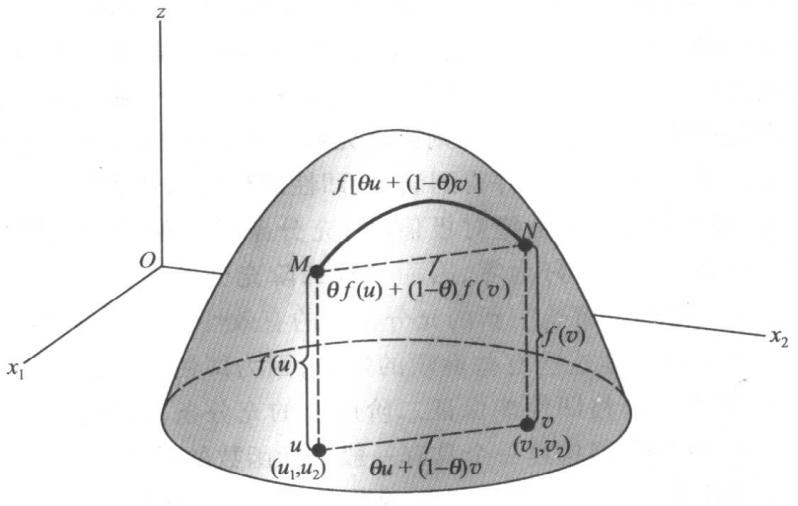
\includegraphics[width=0.475 \linewidth]{pic/strictly_convex_function.png}
    }
%  \hspace{0.1cm} % 两图片之间的距离
  \subfigure[二次连续可微函数的极值与凹凸性]{ 
    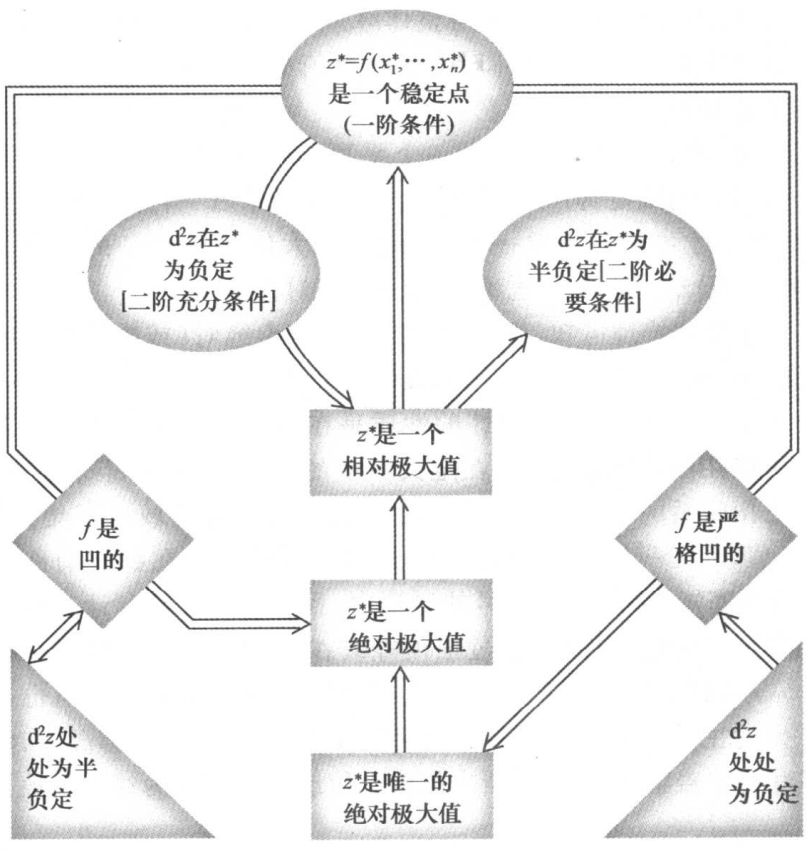
\includegraphics[width=0.475 \linewidth]{pic/quadratic_continuous_differentiable_function.png}
    }
%  \caption{...}
\end{figure}
\noindent
$$
\underbrace{\theta f(u)+(1-\theta) f(v)}_{\text{线段的高度}} 
\left\{\begin{array}{c}\leqslant \\ \geqslant\end{array}\right\}
\underbrace{f\left[\theta u+(1-\theta) v\right]}_{\text{弧的高度}}
\Longleftrightarrow
f(x)\text{为}\left\{\begin{array}{c}\text{凹函数} \\ \text{凸函数}\end{array}\right.
$$
\begin{itemize}
	\item 如果函数\textbf{可微}:
		$$
		f(v)
		\left\{\begin{array}{c}\leqslant \\ \geqslant\end{array}\right\}
		f(u)+f^{\prime}(u)(v-u)
		\Longleftrightarrow
		\text{可微函数}f(x)\text{为}\left\{\begin{array}{c}\text{凹函数} \\ \text{凸函数}\end{array}\right.
		$$
	\item 多个自变量:
		$$
		f(v)\left\{\begin{array}{l}\leqslant \\ \geqslant\end{array}\right\} f(u)+\sum_{j=1}^{n} f_{j}(u)\left(v_{j}-u_{j}\right)
		\Longleftrightarrow
		\text{可微函数}f(\boldsymbol{x})\text{为}\left\{\begin{array}{c}\text{凹函数} \\ \text{凸函数}\end{array}\right.
		$$
	\item 二次连续可微函数:
		\begin{itemize}
			\item \textbf{当且仅当}$\mathrm{d}^2z$处处为$\left\{\begin{array}{l}\text{负}\\\text{正}\end{array}\right\}$半定,$z=f(x_1,x_2,\cdots,x_n)$为$\left\{\begin{array}{c}\text{凹函数} \\ \text{凸函数}\end{array}\right.$	
			\item 当(\textbf{但不是仅当})$\mathrm{d}^2z$处处为$\left\{\begin{array}{l}\text{负}\\\text{正}\end{array}\right\}$定,$z$为\textbf{严格}$\left\{\begin{array}{c}\text{凹函数} \\ \text{凸函数}\end{array}\right.$
		\end{itemize}
\end{itemize}

%
\subsection{凸函数与凸集}
%%
\begin{itemize}
	\item 
	向量\textbf{凸组合}(两个向量的加权平均):
	$\theta u + (1-\theta)v,\quad (0 \leqslant \theta \leqslant 1)$
	\item 
	任意两点$u, v \in S$,当且仅当$w=\theta u+(1-\theta) v \in S$时,$S$为\textbf{凸集}。
\end{itemize}
%%
\begin{figure}[htpb]
  \begin{center}
    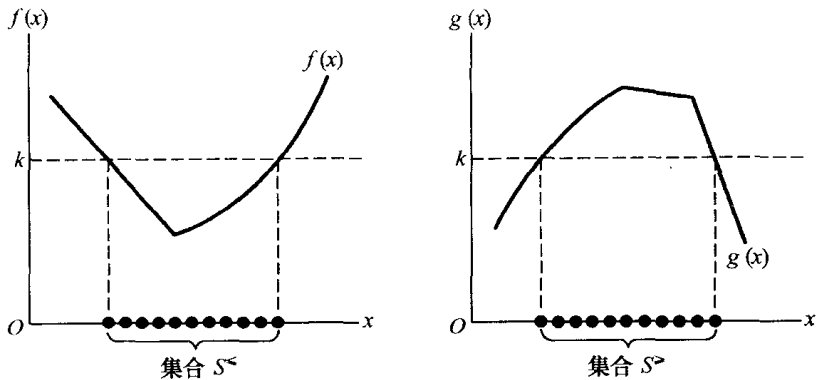
\includegraphics[width=1 \linewidth]
    {pic/convex_set_and_concave_set.png}
%    \caption{凸集与凹集}
  \end{center}
\end{figure}
$$
\left\{\begin{array}{l}
S^{\leqslant} \equiv\{x \mid f(x) \leqslant k\}, \quad[f(x)\text{为凸函数}]
\\
S^{\geqslant} \equiv\{x \mid f(x) \geqslant k\}, \quad[f(x)\text{为凹函数}]
\end{array}\right.
$$

%
\subsection{具有约束方程的最优化}
%%
\subsubsection{一阶条件:\boxed{\text{拉格朗日乘数法}}}
\noindent
目标函数$z$满足约束条件:
$$
\begin{array}{c}
	z=f\left(x_{1}, x_{2}, \cdots, x_{n}\right)
	\\
	\text{s.t.} \quad 
	g\left(x_{1}, x_{2}, \cdots, x_{n}\right)=c
	\\
	\Uparrow
	\\
	(\mathrm{d}g=)
	g_{x_1}\mathrm{d}x_1+g_{x_2}\mathrm{d}x_2+\cdots+g_{x_n}\mathrm{d}x_n=0
	(=\mathrm{d}c)
	\\
	\text{即}\ \mathrm{d}g=0
\end{array}
$$
拉格朗日函数为:
$$
Z=f\left(x_{1}, x_{2}, \cdots, x_{n}\right)+\lambda\left[c-g\left(x_{1}, x_{2}, \cdots, x_{n}\right)\right]
$$
一阶条件为:
$$
\begin{array}{l}
	Z_{\lambda}=c-g\left(x_{1}, x_{2}, \cdots, x_{n}\right)=0 \text{(满足约束条件)} \\
	\left.\begin{array}{l}
		Z_{1}=f_{1}-\lambda g_{1}=0 \\
		Z_{2}=f_{2}-\lambda g_{2}=0 \\
		\cdots \cdots \cdots \cdots \cdots \cdots \\
		Z_{n}=f_{n}-\lambda g_{n}=0
	\end{array}\right\}
	\Rightarrow
	\lambda = 
	\frac{f_{1}}{g_{1}} = \frac{f_{2}}{g_{2}} = \cdots = \frac{f_{n}}{g_{n}} 
\end{array}
$$
\textbf{拉格朗日乘数}$\lambda^{*}$的解释:度量\textbf{目标函数}$Z^{*}$对\textbf{约束条件}的\textbf{敏感性}。
$$
\frac{\mathrm{d} Z^{*}}{\mathrm{d} c} = \lambda^{*}
$$
%%
\subsubsection{二阶条件:\boxed{\text{海塞加边行列式}}}
\noindent
满足线性约束的两个变量的二次型:
$$
\begin{array}{c}
	q=a u^{2}+2 h u v+b v^{2}
	\\
	\text{s.t.} \quad
	\alpha u+\beta v=0
\end{array}
$$
将$q$写成仅有一个变量的函数:
$$
q=a u^{2}-2 h \frac{\alpha}{\beta} u^{2}+b \frac{\alpha^{2}}{\beta^{2}} u^{2}=\left(\alpha \beta^{2}-2 h \alpha \beta+b \alpha^{2}\right) \frac{u^{2}}{\beta^{2}}
$$
当且仅当
$|\bar{H}| 
=
\left|\begin{array}{lll}0 & g_{x} & g_{y} \\ g_{x} & Z_{x x} & Z_{x y} \\ g_{y} & Z_{y x} & Z_{y y}\end{array}\right| 
=
\left|\begin{array}{lll}0 & \alpha & \beta \\ \alpha & a & h \\ \beta & h & b\end{array}\right|
\lessgtr 0
$,
$q(\mathrm{d}z^2)$为
$\left\{\begin{array}{l}\text{正定} \\ \text{负定}\end{array}\right\}$,
且满足$\alpha u+\beta v=0$(即$\mathrm{d}g=0$)

%%
\noindent
\textbf{二阶充分条件}:给定$Z=f(x, y)+\lambda[c-g(x, y)]$,
$|\bar{H}|$为\textbf{正/负}是
稳定值为$z$的\textbf{极大/小值}的\textbf{充分条件}。

%%
$n$个变量:
$$
\begin{array}{c}
	z=f\left(x_{1}, x_{2}, \cdots, x_{n}\right)
	\\
	\text{s.t.} \quad
	g\left(x_{1}, x_{2}, \cdots, x_{n}\right)=c
	\\
	\Uparrow
	\\
	(\mathrm{d} g=) g_{1} \mathrm{~d} x_{1}+g_{2} \mathrm{~d} x_{2}+\cdots+g_{n} \mathrm{~d} x_{n}=0
\end{array}
$$
\textbf{海塞加边行列式}:
$$
|\bar{H}|=
\left|
\begin{array}{ccccc}
	0 & g_{1} & g_{2} & \cdots & g_{n} \\
	g_{1} & Z_{11} & Z_{12} & \cdots & Z_{1 n} \\
	g_{2} & Z_{21} & Z_{22} & \cdots & Z_{2 n} \\
	\cdots &\cdots &\cdots &\cdots &\cdots \\
	g_{n} & Z_{n 1} & Z_{n 2} & \cdots & Z_{n n}
\end{array}
\right|
$$
其\textbf{逐次加边主子式}为:
$$
\left|\bar{H}_{2}\right| \equiv
\left|
\begin{array}{lll}
	0 & g_{1} & g_{2} \\
	g_{1} & Z_{11} & Z_{12} \\
	g_{2} & Z_{21} & Z_{22}
\end{array}
\right|,\quad
\left|\bar{H}_{3}\right| \equiv
\left|
\begin{array}{cccc}
	0 & g_{1} & g_{2} & g_{3} \\
	g_{1} & Z_{11} & Z_{12} & Z_{13} \\
	g_{2} & Z_{21} & Z_{22} & Z_{23} \\
	g_{3} & Z_{31} & Z_{32} & Z_{33}
\end{array}
\right|,\quad
\cdots
$$
当且仅当
$
\left\{\begin{array}{l}
	\left|\bar{H}_{2}\right|,\left|\bar{H}_{3}\right|, \cdots,\left|\bar{H}_{n}\right|<0 \\
	 \left|\bar{H}_{2}\right|>0 , \left|\bar{H}_{3}\right|<0 , \left|\bar{H}_{4}\right|>0, \cdots
 \end{array}\right.
$,
$\mathrm{d}^2 z$为
$
\left\{\begin{array}{l}
	\text{正定}\\
	\text{负定}
\end{array}\right.	
$
满足$\mathrm{d}g=0$。
\newline

%%
\noindent
多重约束下
\begin{itemize}
	\item 拉格朗日函数
	$$
	Z=f\left(x_{1}, \cdots, x_{n}\right)+\sum_{i=1}^{m} \lambda_{j}\left[c_{j}-g^{j}\left(x_{1}, \cdots, x_{n}\right)\right]
	$$
	\item 海塞加边行列式
	$$
	|\bar{H}| \equiv
	\left|\begin{array}{cccccccc}0 & 0 & \cdots & 0 & g_{1}^{1} & g_{2}^{1} & \cdots & g_{n}^{1} \\ 0 & 0 & \cdots & 0 & g_{1}^{2} & g_{2}^{2} & \cdots & g_{n}^{2} \\  0 & 0 & \cdots & 0 & g_{1}^{m} & g_{2}^{m} & \cdots & g_{n}^{m} \\  g_{1}^{1} & g_{1}^{2} & \cdots & g_{1}^{m} & Z_{11} & Z_{12} & \cdots & Z_{1 n} \\ g_{2}^{1} & g_{2}^{2} & \cdots & g_{2}^{m} & Z_{21} & Z_{22} & \cdots & Z_{2 n} \\  g_{n}^{1} & g_{n}^{2} & \cdots & g_{n}^{m} & Z_{n 1} & Z_{n 2} & \cdots & Z_{n n}\end{array} \right|
	$$	
	\item 二阶充分条件:$(n-m)$个加边主子式的代数符号\textbf{相同}(\textbf{交替变换})
	$$\left|\bar{H}_{m+1}\right|,\left|\bar{H}_{m+2}\right|, \cdots,\left|\bar{H}_{n}\right|(=|\bar{H}|)$$
\end{itemize}

%
\subsection{拟凸性与拟凹性(免除检验二阶条件)}
\begin{itemize}
	\item 
		当且仅当函数\ $f$\ 定义域(凸集)中的两点\ $u$\ 和\ $v$,
		且$0<\theta<1$,
		$$
		f(v) \geqslant f(u)
		\Longrightarrow
		f[\theta u+(1-\theta) v]
		\left\{\begin{array}{l} > \geqslant f(u) \\< \leqslant f(v)\end{array}\right.,
		f\text{为}
		\left\{\begin{array}{l}\text{(严格)拟凹} \\ \text{(严格)拟凸}\end{array}\right.
		$$
	\item 
		对于任意常数$k$,当且仅当
		$
		\left\{\begin{array}{l}
		S^{\leqslant} \equiv\{x \mid f(x) \leqslant k\} \\
		S^{\geqslant} \equiv\{x \mid f(x) \geqslant k\} 
		\end{array}\right.
		$
		是凸集,$f(x)$是
		$
		\left\{\begin{array}{l}
			\text{是拟凸的} \\
			\text{是拟凹的}
		\end{array}\right.
		$
	\item 
		对于\textbf{可微函数}
		$f\left(x_{1}, \cdots, x_{n}\right)$定义域中任意两点
		$u=\left(u_{1}, \cdots, u_{n}\right)$
		和$v=\left(v_{1}, \cdots, v_{n}\right)$,
		当且仅当
		$$
		f(v) \geqslant f(u) 
		\Rightarrow
		\left.
		\begin{array}{l}
			\sum_{j=1}^{n} f_{j}(u)\left(v_{j}-u_{j}\right) \\
			\sum_{j=1}^{n} f_{j}(v)\left(v_{j}-u_{j}\right)
		\end{array}
		\right\} 
		\geqslant 0,
		f(x)\text{为}
		\left\{\begin{array}{l}
			\text{拟凹函数} \\
			\text{拟凸函数}
		\end{array}\right.
		$$
		若$z=f\left(x_{1}, \cdots, x_{n}\right)$
		为\textbf{二阶连续可微函数},
		拟凹性和拟凸性可以用函数的一阶导数和二阶导数(整理成加边行列式)的方法检验:
		$$
		|B|=\left|\begin{array}{ccccc}0 & f_{1} & f_{2} & \cdots & f_{n} \\ f_{1} & f_{11} & f_{12} & \cdots & f_{1 n} \\ f_{2} & f_{21} & f_{22} & \cdots & f_{2 n} \\ \cdots &\cdots &\cdots &\cdots &\cdots \\ f_{n} & f_{n 1} & f_{n 2} & \cdots & f_{n n}\end{array}\right|
		$$
		\textbf{拟凹函数}的\textbf{必要条件}:
		$$
		\left|B_{1}\right|=\left|\begin{array}{ll}0 & f_{1} \\ f_{1} & f_{11}\end{array}\right| \leqslant 0, 
		\left|B_{2}\right|=\left|\begin{array}{lll}0 & f_{1} & f_{2} \\ f_{1} & f_{11} & f_{12} \\ f_{2} & f_{21} & f_{22}\end{array}\right|\geqslant 0, 
		\quad \cdots, \quad
		\left|B_{n}\right|=|B|
		\left\{
		\begin{array}{l}
			\leqslant 0 \\
			\geqslant 0
		\end{array}
		\right.
		$$
		$$
		Z_j=f_j-\lambda a_j = 0
		\quad\Rightarrow\quad
		f_j=\lambda a_j = \lambda g_j
		\quad\Rightarrow\quad
		\bigstar \quad \boxed{|B|=\lambda^2|\bar{H}|}
		$$
	\item \textbf{显拟凹函数}
		
		当且仅当
		$
		\underbrace{f(v)>f(u)}_{\text{区别(严格)拟凸拟凹}的} 
		\Longrightarrow
		f[\theta u+(1-\theta) v] > f(u) 
		$,
		$f$为\textbf{显拟凹函数}
\end{itemize}
%%
\begin{figure}[htpb]
  \begin{center}
    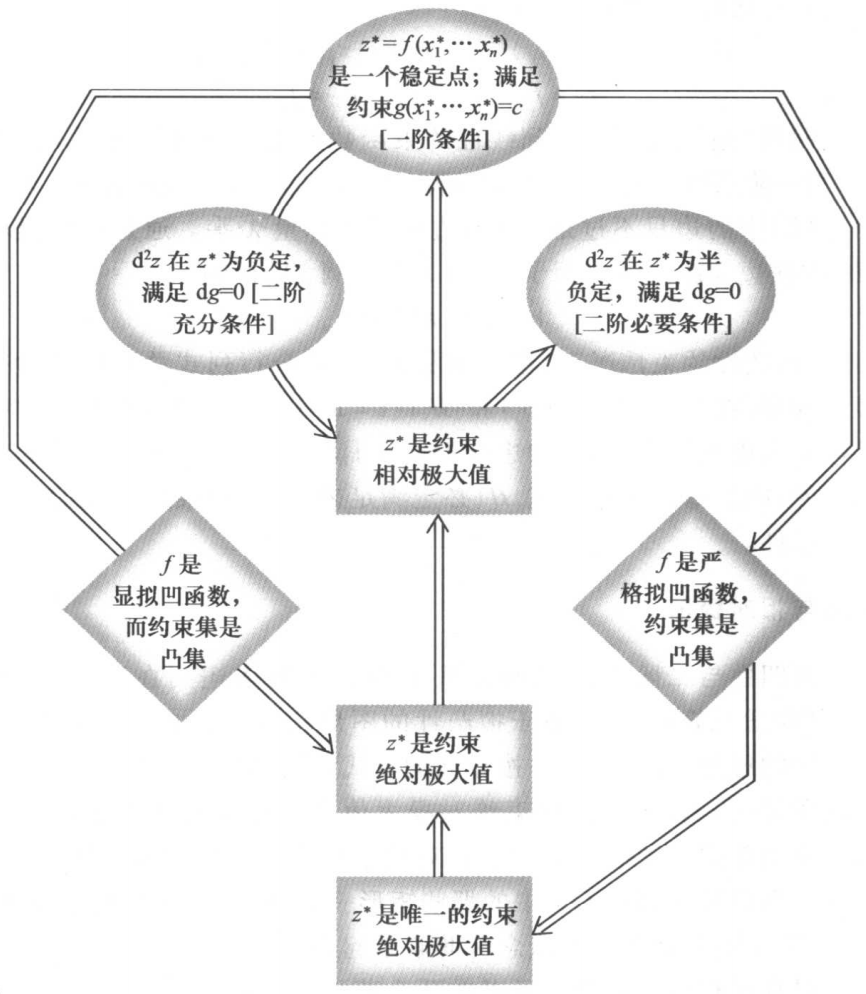
\includegraphics[width=1 \linewidth]
    {pic/constrained_extreme_value.png}
%    \caption{约束极值}
  \end{center}
\end{figure}

%
\subsection{
齐次函数\
$
f\left(j x_{1}, \cdots, j x_{n}\right)=j^{r} f\left(x_{1}, \cdots, x_{n}\right)
$
}
%%
\textbf{生产函数}为线性齐次:
$Q = f(L, K)\quad [=L\phi(k)]$
\begin{itemize}
	\item $
		\operatorname{APP}_L \equiv \frac{Q}{L} = f(\frac{K}{L},1)=f(k,1)=\phi(k), 
		\quad
		\operatorname{APP}_K \equiv \frac{Q}{K}=\frac{Q}{L}\frac{L}{K}=\frac{\phi(k)}{k}
		$
	\item $
		\frac{\partial k}{\partial K}=\frac{\partial}{\partial K}\left(\frac{K}{L}\right)=\frac{1}{L}, 
		\quad 
		\frac{\partial k}{\partial L}=\frac{\partial}{\partial L}\left(\frac{K}{L}\right)=\frac{-K}{L^{2}}
		$
		$$
		\begin{aligned} \operatorname{MPP}_{K} \equiv \frac{\partial Q}{\partial K} 
		& =\frac{\partial}{\partial K}[L \phi(k)] 
		 =L \frac{\partial \phi(k)}{\partial K}
		\\ & =L \frac{\mathrm{d} \phi(k)}{\mathrm{d} k} \frac{\partial k}{\partial K} 
		 =L \phi^{\prime}(k)\left(\frac{1}{L}\right)=\phi^{\prime}(k)
		\end{aligned}
		$$
		$$
		\begin{aligned} 
		\mathrm{MPP}_{L} \equiv \frac{\partial Q}{\partial L} & =\frac{\partial}{\partial L}[L \phi(k)] 
		\\ & =\phi(k)+L \frac{\partial \phi(k)}{\partial L} 
		 =\phi(k)+L \phi^{\prime}(k) \frac{\partial k}{\partial L} 
		\\ & =\phi(k)+L \phi^{\prime}(k) \frac{-K}{L^{2}} 
		 =\phi(k)-k \phi^{\prime}(k)
		\end{aligned}
		$$
	\item \textbf{欧拉定理}
		$$
		K \frac{\partial Q}{\partial K}+L \frac{\partial Q}{\partial L} \equiv Q
		$$
\end{itemize}

%%
$\bigstar$ \quad 推广:包含$n$个变量的\textbf{线性齐次函数}\
$y=f\left(x_{1}, x_{2}, \cdots, x_{n}\right)$
$$
y=x_{1} \phi\left(\frac{x_{2}}{x_{1}}, \frac{x_{3}}{x_{1}}, \cdots, \frac{x_{n}}{x_{1}}\right)\quad [ \text{一次齐次性} ]
$$
$$
\sum_{i=1}^{n} x_{i} f_{i} \equiv y
\quad [\text{欧拉定理}]
$$
$$
y=x_{1}^{r} \phi\left(\frac{x_{2}}{x_{1}}, \frac{x_{3}}{x_{1}}, \cdots, \frac{x_{n}}{x_{1}}\right) 
\quad [r \text{次齐次性} ]
$$
$$
\sum_{i=1}^{n} x_{i} f_{i} \equiv r y
\quad [\text{修正的欧拉定理}]
$$

%
\subsection{非线形规划}
\subsubsection{一阶条件:库恩塔克条件}

%%%%%%%%%%%%%%%%%%%%%%%%%%
\newpage
\section{动态分析}


\end{CJK*}
\bigskip
\end{document}